\subsection{Uso del Triac y Diac}
    Como en el presente trabajo práctico, se utilizará un circuito de
    disparo compuesto con un triac y un diac, se explciara brevemente
    de que trata cada dispositivo y como se forma el circuito de la placa
    propia del TP. 
    
    \subsubsection{Diac}
        EL Diac es un dispositivo semiconductor, posee 4 capas y dos terminales de conexión
        como se observa en la Figura \ref{fig:EstrucDiac}, con la particularidad de poder 
        circular corriente en ambos sentidos cuando es activado. La conduccion en el diac,
        ocurre cuando se alcanza el voltaje de ruptura \(V_{BO}\) en cualquiera de los dos 
        sentidos; Y se apaga cuando al corriente se reduce por debajo del voltaje mencionado. 
        La curva del dispositivo se observa en la Figura \ref{fig:CurvaDiac} 

        \begin{figure}[H]
            \centering
            \begin{subfigure}[ht]{0.48\textwidth}
              \frame{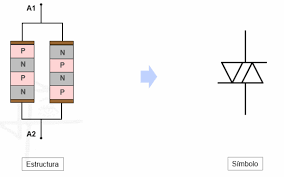
\includegraphics[width=\textwidth]{Imagenes/MarcoTeorico/TRIACyDIAC/DIAC2.png}}
              \caption{Estructura y sumbolo del DIAC.}
              \label{fig:EstrucDiac}
            \end{subfigure}
            \hfill 
            \begin{subfigure}[ht]{0.48\textwidth}
              \frame{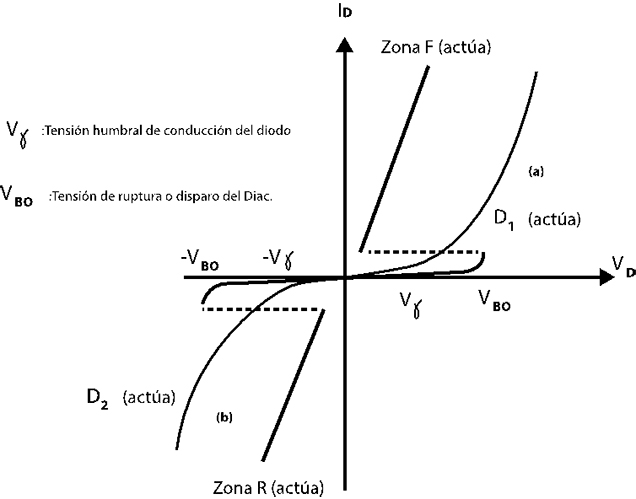
\includegraphics[width=\textwidth]{Imagenes/MarcoTeorico/TRIACyDIAC/curvaDIAC.jpg}}
              \caption{Curva de trabajo del DIAC.}
              \label{fig:CurvaDiac}
            \end{subfigure}
        \end{figure}

    \subsubsection{TRIAC}
        
        El Triac es como un Diac pero con un terminal de compuerta G (\textit{gate}), 
        el cual le permite ser disparado por un pulso de corriente en dicha terminal.
        A digferencia del Diac, no requiere de un voltaje de ruptura para iniciar 
        la conducción. Basicamente, el triac se lo puede pensar como dos SCR conectados en 
        paralelo, en direccones opuestas con un terminal en común G, como se observa en La
        Figura \ref{fig:EstrucTriac}.
        Este dispositivo es capaz, tambien como el Diac, de conducir corriente en ambos
        sentidos segun la polaridad de vltaje que tenga entre sus bornes. La curva de trabajo
        del mismo se observa en la Figura \ref{fig:CurvaTriac}   
    
        \begin{figure}[H]
            \centering
            \begin{subfigure}[ht]{0.48\textwidth}
              \frame{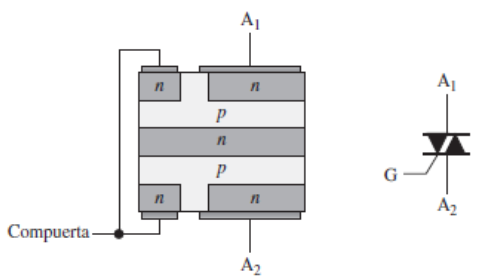
\includegraphics[width=\textwidth]{Imagenes/MarcoTeorico/TRIACyDIAC/simboloTRIAC.png}}
              \caption{Estructura y sumbolo del TRIAC.}
              \label{fig:EstrucTriac}
            \end{subfigure}
            \hfill 
            \begin{subfigure}[ht]{0.48\textwidth}
              \frame{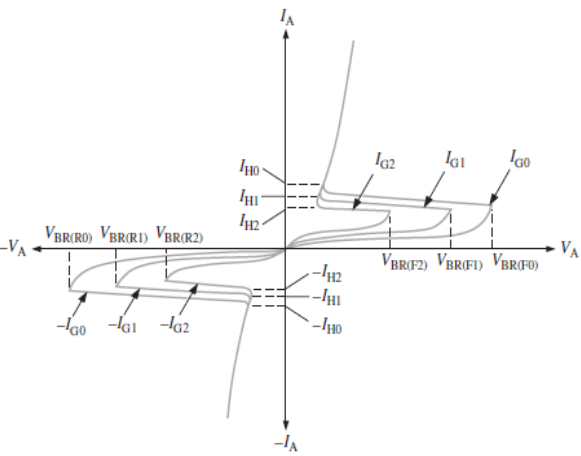
\includegraphics[width=\textwidth]{Imagenes/MarcoTeorico/TRIACyDIAC/curvaTRIAC.png}}
              \caption{Curva de trabajo del TRIAC.}
              \label{fig:CurvaTriac}
            \end{subfigure}
        \end{figure}

    \subsubsection{Circuito de disparo con Triac y Diac}
        
        Para este trabajo práctico se utilzará, el siguiente circuito de disparo 
        de triac con diac, (\textit{Dimer}) comos e observa en al Figura 
        \ref{fig:CircuitoTriacDiac}

        \begin{figure}[H]
            \centering
            \frame{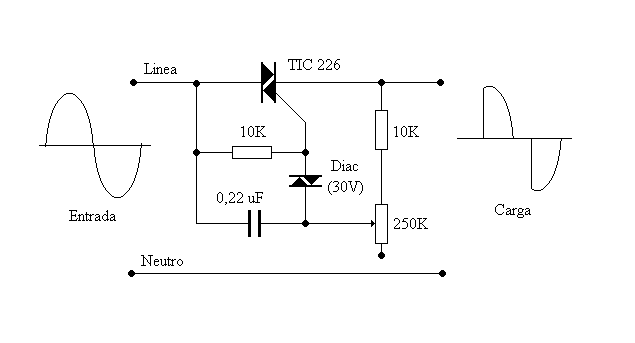
\includegraphics[width=0.45\textwidth]{Imagenes/MarcoTeorico/TRIACyDIAC/Esquema_Circuito_Angulo_Disparo.png}}
            \caption{Circuito Dimer con Triac y Diac.}
            \label{fig:CircuitoTriacDiac}
          \end{figure}

        EL potenciometro de 250~K\(\Omega\), lo que hace es regular el tiempo de carga del condensador 
        de 0.22~\(\mu F\), el cual es el encargado de entregar la tensión de ruptura para que el diac
        conduzca. Una vez que el diac conduce, deja pasar una tensión la cual polariza al triac
        a travez de su terminal G. El triac no conducira, hasta que, se le de un pulso de 
        activacion en el gate, y dejara de conducir cuando la onda seoindal cruce por cero.
        Para que vuelva a conducir, el diac es polarizado en el otro sentido y de esta manera, 
        se genera un nuevo pulso en el gate del triac y el mismo conducira en el otro semisiclo
        de la onda seidal. Como vemos en el esquematico entre el terminal G del triac y el diac, 
        tenemos una resitencia lmitadora de corrinte para el terminal G de 10~K\(\Omega\).
        Por ultimo, la otra resistencia de 10~K\(\Omega\), conectada en serie con el potenciometro, 
        es utilizada como limitador de corriente para el cicuito de disparo. 
